\chapter{Check routines for reinforced concrete}
\section{Introduction}
This chapter describes the routines that can be used to check the design following the specifications of different design codes.

\section{Verification of RC sections}

\subsection{Sections definition}



\subsection{Limit State at Failure under normal stresses verification}

\subsubsection{lanzaCalculoTNFromXCData}
This function carries out the verification of the limit state at failure under nornal stresses. It takes as input the internal forces and bending moments calculated for the shell elements for every ULS combinations, the sections definition and the interaction diagrams to be employed.

The function returns two files with the verification results:
{\tt outputFileName.py}: XC file that assigns each shell element the capacity factor (worst-case) {\tt FCC} calculated for reinforcement in directions 1 and 2, together with the concomitant axial force and bending moments {\tt N My Mz}.
{\tt outputFileName.py}: \LaTeX\  file containing a table with the following items:

\begin{center}
\begin{tabular}{ccccccc}
\multicolumn{7}{l}{\textbf{Section 1}} \\
\\
Element & Section & ULS & Axial & Bending & Bending & Capacity \\
number  & name & name & force NCP1 & moment MyCP1 & moment MzCP1 & factor FCCP1 \\
\hline
\multicolumn{7}{l}{\ldots\ \ldots\ \ldots} \\
\\
\multicolumn{7}{l}{\textbf{Section 2}} \\
\\
Element & Section & ULS & Axial & Bending & Bending & Capacity \\
number  & name & name & force NCP2 & moment MyCP2 & moment MzCP2 & factor FCCP2 \\
\hline
\multicolumn{7}{l}{\ldots\ \ldots\ \ldots} \\
\\

\end{tabular}
\end{center}

\begin{figure}[h]
\centering
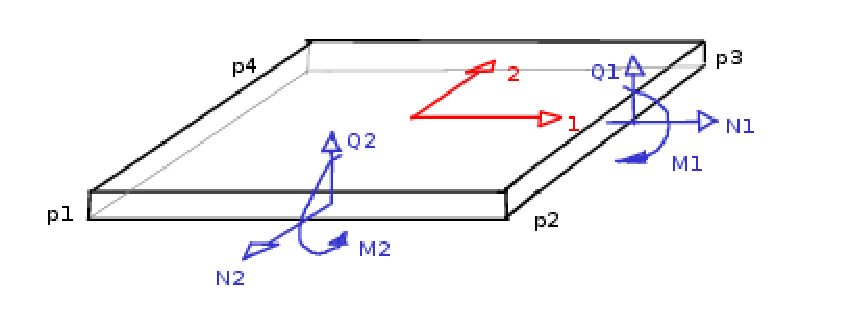
\includegraphics[width=100mm]{materials/figures/signosEsfuerzos}
\caption{Positive directions of forces and moments in shell elements}\label{shell_forces_moments}
\end{figure}

 
\begin{verbatim}
from materials.xLamina import calculo_tn
calculo_tn.lanzaCalculoTNFromXCData(preprocessor,analysis,intForcCombFileName,outputFileName, 
mapSectionsForEveryElement,mapSectionsDefinition, mapInteractionDiagrams)
\end{verbatim}
\begin{paramFuncTable}
\preprocessor{} \\
\analysis{} \\
\intForcCombFileName{ULS under normal stresses}{ULS}\\
\outputFileName{}\\
\mapSectionsForEveryElement{} \\
\mapSectionsDefinition{} \\
\mapInteractionDiagrams{} \\
\end{paramFuncTable}


\subsection{Limit State of Failure due to shear verification}
This function carries out the verification of the limit state at failure under nornal stresses. It takes as input the internal forces and bending moments calculated for the shell elements for every ULS combinations, the sections definition and the interaction diagrams to be employed.

The function returns two files with the verification results:

{\tt outputFileName.py}: XC file that assigns each shell element the capacity factor (worst-case) {\tt FCC} calculated for reinforcement in directions 1 and 2, together with the concomitant forces and moments {\tt N My Mz  Vy Vz } and the ultimate shear forces and moment {\tt Mu Vcu Vsu Vu }
{\tt outputFileName.py}: \LaTeX\  file containing a table with the following items:

\begin{footnotesize}
\begin{center}
\begin{tabular}{ccccccccccc}
\multicolumn{7}{l}{\textbf{Section 1}} \\
\\
Element & Section & ULS  & Axial      & Bending      & Bending      & Cracking       & Shear       & Shear       & Ultimate & Capacity \\
number  & name    & name & force      & moment       & moment       & moment & force       & force       & shear    & factor       \\
        &         &      &       NCP1 &        MyCP1 &        MzCP1 & MuCP1          &       VyCP1 &       VyCP1 & force VuCP1 & FCCP1 \\
\hline
\multicolumn{7}{l}{\ldots\ \ldots\ \ldots} \\
\\
\multicolumn{7}{l}{\textbf{Section 2}} \\
\\
Element & Section & ULS  & Axial      & Bending      & Bending      & Cracking       & Shear       & Shear       & Ultimate & Capacity \\
number  & name    & name & force      & moment       & moment       & moment & force       & force       & shear    & factor       \\
        &         &      &       NCP2 &        MyCP2 &        MzCP2 & MuCP2          &       VyCP2 &       VyCP2 & force VuCP2 &       FCCP2 \\


\hline
\multicolumn{7}{l}{\ldots\ \ldots\ \ldots} \\
\\

\end{tabular}
\end{center}
\end{footnotesize}


\begin{verbatim}
from materials.xLamina import calculo_v
calculo_v.lanzaCalculoV(preprocessor,analysis,intForcCombFileName,outputFileName, 
mapSectionsForEveryElement,mapSectionsDefinition,mapInteractionDiagrams,
procesResultVerifV)
\end{verbatim}

\begin{paramFuncTable}
\preprocessor{} \\
\analysis{} \\
\intForcCombFileName{ULS due to shear}{ULS}\\
\outputFileName{}\\
\mapSectionsForEveryElement{} \\
\mapSectionsDefinition{} \\
\mapInteractionDiagrams{} \\
\procesResultVerifV{} \\
\end{paramFuncTable}


\subsection{Cracking limit state verification}
\begin{verbatim}
from materials.xLamina import calculo_fis
calculo_fis.lanzaCalculoFISFromXCDataPlanB(preprocessor,analysis,intForcCombFileName,
outputFileName, mapSectionsForEveryElement,mapSectionsDefinition,
procesResultVerifFIS)
\end{verbatim}
\begin{paramFuncTable}
\preprocessor{} \\
\analysis{} \\
\intForcCombFileName{cracking limit state}{quasi permanent SLS or frequent SLS}\\
\outputFileName{}\\
\mapSectionsForEveryElement{} \\
\mapSectionsDefinition{} \\
\mapInteractionDiagrams{} \\
\procesResultVerifFIS{} \\
\end{paramFuncTable}


\section{Verification of beam sections}

\section{Punching shear calculation}

\subsection{Punching shear calculation according to EC2}
